\documentclass[dissertation,copyright]{uathesis}
\usepackage[]{graphicx}\usepackage[]{color}
%% maxwidth is the original width if it is less than linewidth
%% otherwise use linewidth (to make sure the graphics do not exceed the margin)
\makeatletter
\def\maxwidth{ %
  \ifdim\Gin@nat@width>\linewidth
    \linewidth
  \else
    \Gin@nat@width
  \fi
}
\makeatother

\definecolor{fgcolor}{rgb}{0.345, 0.345, 0.345}
\newcommand{\hlnum}[1]{\textcolor[rgb]{0.686,0.059,0.569}{#1}}%
\newcommand{\hlstr}[1]{\textcolor[rgb]{0.192,0.494,0.8}{#1}}%
\newcommand{\hlcom}[1]{\textcolor[rgb]{0.678,0.584,0.686}{\textit{#1}}}%
\newcommand{\hlopt}[1]{\textcolor[rgb]{0,0,0}{#1}}%
\newcommand{\hlstd}[1]{\textcolor[rgb]{0.345,0.345,0.345}{#1}}%
\newcommand{\hlkwa}[1]{\textcolor[rgb]{0.161,0.373,0.58}{\textbf{#1}}}%
\newcommand{\hlkwb}[1]{\textcolor[rgb]{0.69,0.353,0.396}{#1}}%
\newcommand{\hlkwc}[1]{\textcolor[rgb]{0.333,0.667,0.333}{#1}}%
\newcommand{\hlkwd}[1]{\textcolor[rgb]{0.737,0.353,0.396}{\textbf{#1}}}%
\let\hlipl\hlkwb

\usepackage{framed}
\makeatletter
\newenvironment{kframe}{%
 \def\at@end@of@kframe{}%
 \ifinner\ifhmode%
  \def\at@end@of@kframe{\end{minipage}}%
  \begin{minipage}{\columnwidth}%
 \fi\fi%
 \def\FrameCommand##1{\hskip\@totalleftmargin \hskip-\fboxsep
 \colorbox{shadecolor}{##1}\hskip-\fboxsep
     % There is no \\@totalrightmargin, so:
     \hskip-\linewidth \hskip-\@totalleftmargin \hskip\columnwidth}%
 \MakeFramed {\advance\hsize-\width
   \@totalleftmargin\z@ \linewidth\hsize
   \@setminipage}}%
 {\par\unskip\endMakeFramed%
 \at@end@of@kframe}
\makeatother

\definecolor{shadecolor}{rgb}{.97, .97, .97}
\definecolor{messagecolor}{rgb}{0, 0, 0}
\definecolor{warningcolor}{rgb}{1, 0, 1}
\definecolor{errorcolor}{rgb}{1, 0, 0}
\newenvironment{knitrout}{}{} % an empty environment to be redefined in TeX

\usepackage{alltt}
\newcommand{\SweaveOpts}[1]{}  % do not interfere with LaTeX
\newcommand{\SweaveInput}[1]{} % because they are not real TeX commands
\newcommand{\Sexpr}[1]{}       % will only be parsed by R


%\documentclass[dissertation,CC-BY]{uathesis}
%\documentclass[dissertation,CC-BY-SA]{uathesis}
%documentclass[dissertation,CC-BY-ND]{uathesis}
%\documentclass[thesis]{uathesis}
%\documentclass[document]{uathesis}

% Package Usage
% These are the packages that we need
\usepackage{booktabs}
\usepackage{graphicx}
\usepackage{natbib}			% natbib is available on most systems, and is
					% terribly handy.
					
%May need to remove! Trying to fix nocite{*} biblography problem:
					% If you want to use a different Bibliography package, 
					% you should be able to, just change this
					% and the \bibliographystyle command below.  Be warned
					% that you may need to do a little hacking to get
					% the REFERENCES item to show up in your TOC.

% Compatibility with the AASTEX package 
% of the American Astronomical Society.
%\usepackage{deluxetable}		% Allows use of AASTEX deluxe tables
%\usepackage{aastex_hack}		% Allows other AASTEX functionality.

% These are other packages that you might find useful.
% For controlling the fonts, see
% http://www.math.uiuc.edu/~hartke/computer/latex/survey/survey.html
% The following is a nice font set:
%\usepackage{mathtime}			% Times for letters; Belleek math.
%
\usepackage{wrapfig}

\newenvironment{lydiawrapfigure}
 {%
%  \setlength{\intextsep}{0pt}% <--- Wrong!
  \setlength{\columnsep}{15pt}%
  \wrapfloat{figure}%
 }
 {\endwrapfloat}
 
\usepackage{caption}
\usepackage{subcaption}
\usepackage{tipa}
\usepackage{color,soul}
\usepackage{url}
\usepackage{blindtext}
\usepackage[inline]{enumitem}
\usepackage{breakurl}
\usepackage{mathtools}
\usepackage{amsmath}			% AMS Math (advanced math typesetting)
%\usepackage{lscape}			% Used for making fitting large tables in by putting them landscape
%\usepackage{refs}			
%
% If you are using hyper-ref (recommended), this command must go after all 
% other package inclusions (from the hyperref package documentation).
% The purpose of hyperref is to make the PDF created extensively
% cross-referenced.

%Also works! Change dvips to driverfallback=dvips.
\usepackage[driverfallback=dvips,bookmarks,colorlinks=true,urlcolor=black,linkcolor=black,citecolor=black]{hyperref}


%Works!
%\usepackage[pdftex,bookmarks,colorlinks=true,urlcolor=black,linkcolor=black,citecolor=black]{hyperref}
%HERE IS THE THING THAT NEEDS TO CHANGE TO GET LATEX TO WORK WITH RSTUDIO. USE pdftex instead of dvips.

% Set up some values.
\completetitle{Working Title: An approach to automatic and human speech recognition using ear-recorded speech.}
\fullname{Samuel John Charles Johnston}			% Grad college wants your full name here.
\degreename{Doctor of Philosophy}	% Title of your degree.



\begin{document}
%set_parent(‘/Users/mwilli/Documents/Spring_2017/Dissertation_Document/Dissertation_Working_Directory_Draft/Dissertation_Main.Rnw')



 



\chapter{Automatic Speech Recognition of Ear-Recorded Speech\label{chapter3}}


\section{Introduction}

The automatic recognition of human speech by a computer has been a subject of interest spanning decades.  Humans first and foremost communicate their ideas via speech and human language, and teaching computers to be able to take verbal instructions would make interaction with them much easier for a majority of the population, particularly the elderly and disabled.  Since this seemingly simple task has been a subject of much study for over half a century, and is only recently gaining much success, it will be important to briefly discuss the reasons for the challenges, traditional ways of dealing with them, and more recent successes.

Despite these successes, challenges still remain when there is noise in the signal.  As before, it is important to understand the mechnics and acoustics of why this proves to be a challenge for automatic speech recognition (ASR), and traditional methods of dealing with this as well as more modern techniques.

% Insert bit about it being still not perfect?

In the previous chapter, data was collected using a novel technique aimed to overcome the difficulty of accurately perceiving speech in a noisy environment, for recognition both by computer (ASR) or by human speech perception.  This collected data will be used in an experiment using a standard open source ASR system with a standard, open source acoustic model.

\section{Background}
\label{chap3:background}

% Things to hit on:
% - Base-level Acoustics-to-Features
% - Traditional general ASR mechanics?
% - Current methods of ASR (Cutajar + more recent)
% - Outline problem of noise in the signal
% - Traditional methods of filtering noise out of the signal
% - Previous methods of ASR in noise
% -- Issues with these traditional methods (of removing noise and ASR in noise)
% - Current methods of ASR in noise (Li 2014, and more current)
% -- Multiple Microphones and Beamforming
% -- Other methods??  Look at current CHiME challenge papers
% - Try to find continued issue with electronically identifying speech in noise
% - Emphasize unpredictability of noise, and unknown amplitude - how ear-recorded speech may be able to `protect' against this unpredicatability

% The basics of the acoustics of speech was discussed at the beginning of Chapter 2\ref{chapter2}.  As a recap, speech contains voiced and voiceless sounds.  The voiceless sounds are generally produced by turbulence - air moving rapidly through a small openning in the vocal tract.  The voiced sounds are more complex, and contain harmonics (acoustic energy focused in very narrow bands of frequency).  Certain harmonics (out of the full set of harmonics in the voiced signal) contain more energy than the other harmonics; these regions in the frequency spectrum with harmonics containing greater energy are called formants, and this is where much of the speech information comes from.
% 
% The human auditory system does a remarkable job of finding these acoustic features and interpreting them, but a computer does not have an inherent auditory system and (as of now) needs to be told what to look for.  Simply put, via a microphone, computers receive a series of digits (numbers) which correspond to the amount of pressure at a given point in time.  
% %
% \begin{wrapfigure}{L}{0.5\textwidth}
% \centering
% 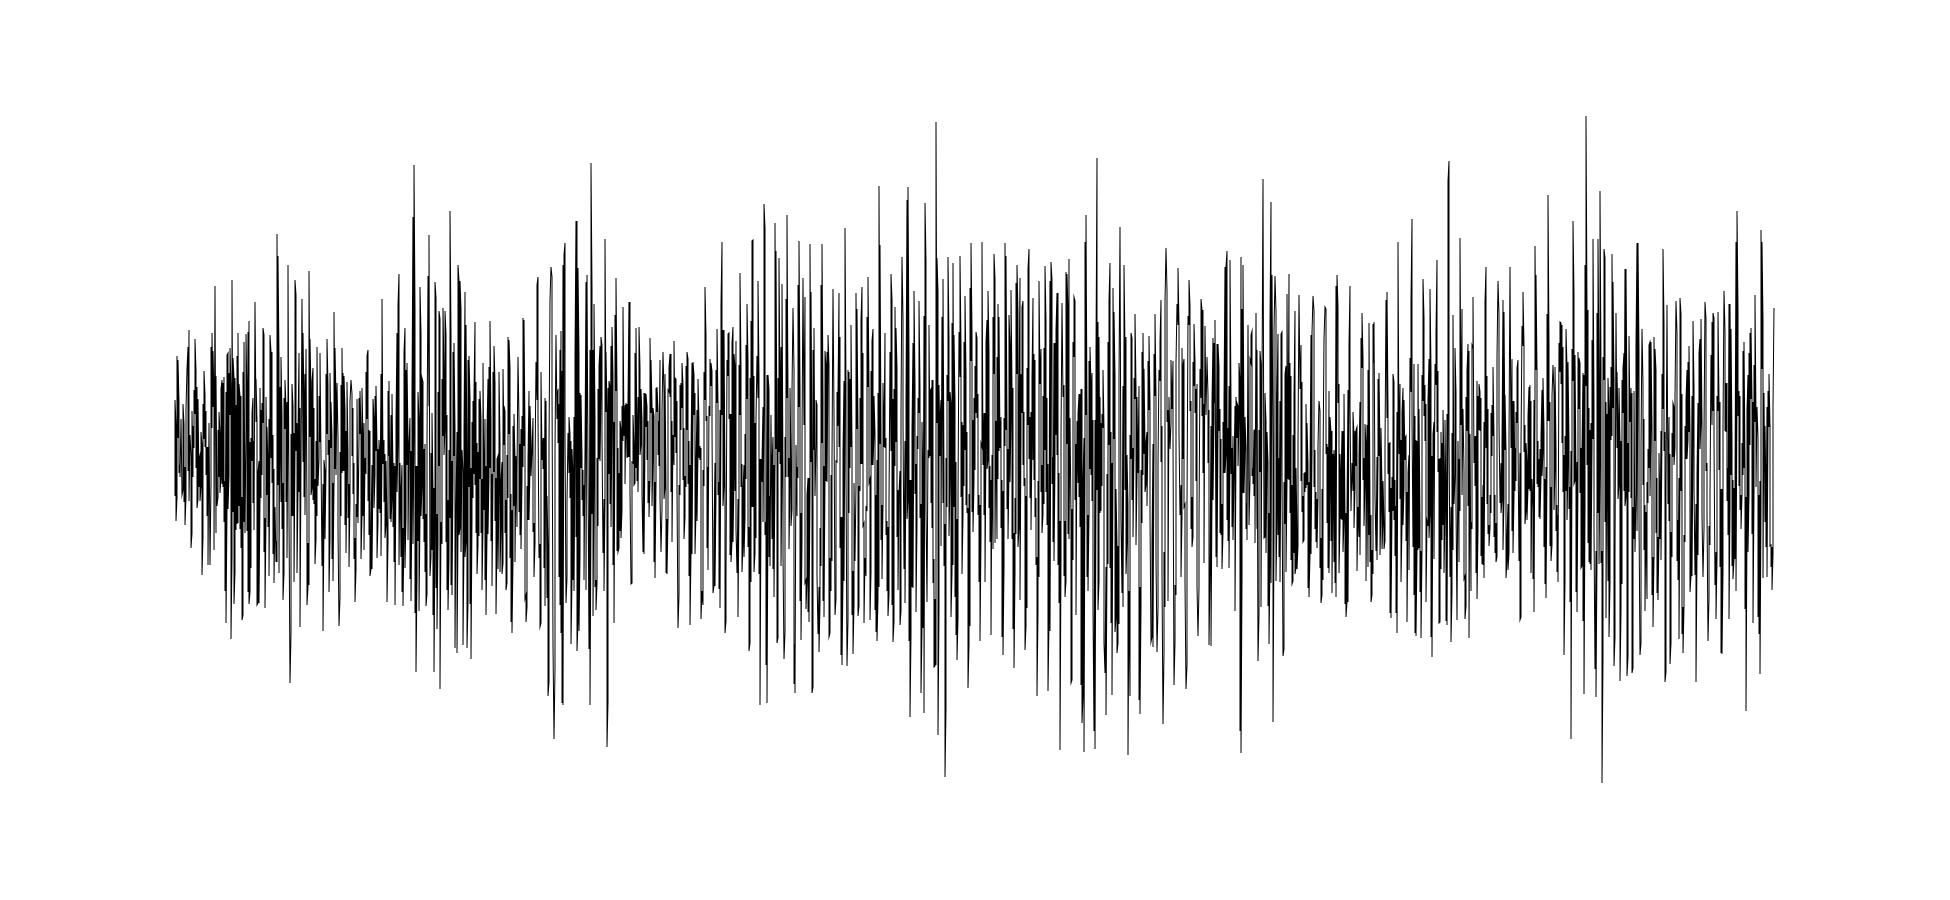
\includegraphics[width=0.45\textwidth]{figure/single-channel-animals.png}
%   \caption{A waveform graph representing the high and low pressure fluctuations that comprise sound.}
%   \label{fig:waveform}
% \end{wrapfigure}

While there are more than 30 years of research involving ASR, and nearly as many working with speech in noisy environments, it is impossible to touch on all techniques in this very brief overview.  Therefore, only several areas of research in noise-robust ASR will be discussed pertaining to the present research.

[Present the problem with function using $x_\textit{t}$ and $y_\textit{t}$, mention reverberation.  Can mention LATER that ear recording elimnates reverberation, introduces OE `reverberation' (though not really reverberation in the same sense), but (c.f. Ch2) this is highly predictable.  Also mention here that phase is rarely accounted for, and is normally assumed out of the equation.]

Equation \ref{eq:basic} is often used to represent the combination of speech and noise,
\begin{equation}\label{eq:basic}
y = x * h + n
\end{equation}
where $x$ is the clean speech signal, $h$ is any convolution (ie. room reverberation, microphone channel warp), $n$ is additive noise, and $y$ is the noisy speech signal.

Multi-style training, what it is (training with multiple types of noise) - it is ineffective.  Older - paper cited was written in 1987. \cite{li:14}, \cite{lippmann:87}.

Noise robustness techniques may be categorized by (a) the kind of observation models used, (b) according to whether an explicit or an implicit distortion model is used, and (c) according to whether or not prior knowledge about distortion is employed to learn the relationship between $x_\textit{t}$ and $y_\textit{t}$ (\cite{li:14}).

%Feature Domain space vs Model Domain space compensation

Feature space is the part of the ASR process where an acoustic vector is transformed into `features' about the acoustic signal that the ASR model will receive as input.  Model space, imperatively, then, comes after Feature space in the ASR process, and encompasses the acoustic model parameters, methods of training the model, etc.

Noise can be accounted for in either or both domains.  In the feature domain, noise is dealt with prior to the sending the features to the acoustic model.  These noise reduction processes intend to enhance the signal before it reaches the model.  This is mostly done without altering the acoustic model parameters, resulting in low computation cost.

In the model space, acoustic parameters themselves can be modified in accordance with the noisy signal.  This generally results in high computation cost when training the acoustic model.  There is normally a trade-off of computation and performance, with Model Domain space alterations generally yielding higher performance improvement (\cite{li:14}).

In the feature domain space, there are a number of techniques, including (a) noise-resistant features, (b) feature normalization, and  (c) feature compensation.  Noise resistant features are, quite simply, features in the acoustic signal which are not sensitive to environmental changes.  Many methods of deriving these features have been proposed that incorporate features of the human auditory system, including Perceptual linear prediction (\cite{hermansky:85}), which aims to replicate \textbf{XXXX}, and Relative Spectral processing (RASTA) applied to Perceptual Linear Prediction (\cite{hermansky:92}), making perceptual linear prediction less sensitive to slow varying speech information, and more sensitive to the quick-varying transitions of speech (\cite{story:10}).  \textbf{ALSO \cite{kim:99}, mimicking XXX}. These methods are quite effective at dealing with short-term, stationary, additive noise (\cite{zhang:17}).  More recent methods include SPARK (\cite{fazel:12}), which mimics \textbf{XXXX}, (\cite{moritz:15}), which mimics \textbf{XXXXX}.  These methods generally outperform normal MFCC methods. Difficulties utilizing these methods include that it is difficult to determine the parameters.  Also the generation of these features can be quite complex, preventing widespread usage with other techniques, and difficulty deriving a relation between clean and noisy speech (which makes explicit distortion modelling difficult).

Feature normalization generally involves normalizing cepstral feature vectors in the form of cepstral mean normalization (CMN) and cepstral mean and variance normalization (CMVN).  CMN invovles finding the mean values out of all cepstral vectors (\cite{atal:74}).  All cepstral vectors are then normalized, such that the mean cepstral value becomes zero.  This is primarily used to eliminate reverberation and channel-related distortion, but signals with noise and no channel distortion also see improvement (\cite{droppo:08}).  ``CMVN normalizes the mean and covariance together'' (\cite{li:14}, 752), yielding improved performance on speech data with additive noise.
These methods do not work in real-time, however, as they require cepstral vectors from the entire utterance in order to calculate a mean.

Feature compensation actually attempts to remove the noise from the noisy speech signal, allowing for use of traditional features. Spectral subtraction (\cite{boll:79} is an older and intuitive method of removing noise by turning the linear signal into the spectral domain, subtracting a noise spectrum from a noisy speech spectrum, leaving the clean speech spectrum.  This is then converted back into the series of samples that derive the clean speech spectrum.  This is performed all along the waveform.  The noise can be estimated by looking at sections of the observed signal that do not contain speech information.  

This method still comes with several problems (\cite{li:14}). First and foremost, it is difficult to detect the location of speech in the signal in a noisy environment, which consequently affects the ability to accurately compute a noise average. It also requires relatively stationary, slow-variation noise, as noise that changes quickly very possibly has a different average spectrum during the portion of the signal containing speech than the portion of the signal in which it was calculated.  Furthermore, this is only an average of the noise, and not exactly the noise itself; this subtraction can inadvertently have an additive noise effect by producing extraneous acoustic artifacts in the ``clean'' signal which were not there to begin with (\cite{berouti:79})

Weiner filtering (\cite{weiner:79}) is another method used to remove noise from a signal.  As opposed to spectral subtraction, however, this is a linear filter that works without the need to convert the signal into spectra.  However, this method also requires an estimation of the noise.  Furthermore, it does not do well in very low SNR enviroments, as it generally results in suppression and dampening of the entire signal (\cite{li:14}).

More standard, is the ``advanced front-end'' (AFE) ensemble proposed in \cite{etsi:02}.  It yields more than 50\% improvement over standard MFCC features alone, and has become a frequent baseline for comparison in noisy ASR research.  It is composed of three separate `tools': two stage Mel-warped Weiner filtering, SNR-dependant waveform processing, and blind equalization (cf. \cite{argawal:99,macho:02;macho:01;mauuary:98}, respectively.



Most of the heavy work is performed by the Mel-warped Weiner filtering (\cite{li:14}).  This differs from the more standard Weiner filter in that it uses \textbf{Mel Weiner filtering???}, which is performed once, and then a second time to remove residual noise.  SNR-dependant waveform processing (SDWP) assumes that the noise is relatively constant, whereas the speech signal will cause variation in the amplitude of the signal.  SDWP uses this assumption to dampen portions of the signal with a relatively low SNR (ie, speech-less) compared with the high SNR (ie, speech-bearing) portions of the signal, which are boosted.  Blind equalization serves to eliminate convolutional (ie. reverberant) distortion from the signal.

Model domain compensation usually involves adapting an existing acoustic model (presumably trained on relatively clean speech) to enable recognition of more noisy features.  Most popularly, variations of maximum likelihood linear regression (MLLR, \cite{leggetter:95}) are used to adjust the gaussian component vector means and the covariance parameters.  A slight variation in the caculation allows these transforms to be applied to the features themselves (feature-space MLLR, or fMLLR, \cite{gales:98}), moving this method into an on-line feature space tranformation.



Another tool used is the exploitation of any prior knowledge about the distortion (\cite{li:14}); this is prior knowledge that is utilized during the training stage, not knowledge about the noise during the testing stage.  Some methods include learning the mapping between noisy and non-noisy pairs of acoustic signals.  This mapping is then extended to novel noisy utterances during testing.  This is used in feature domain space to enhance a noisy speech feature to then send to the model.  

Other methods utilze mutliple acoustic models, each trained on data from different environments and different noises and different SNRs.  The means and covariance matrices of each of these models are stored, and during recognition, the most appropriate model is chosen to use to decode the signal in question.  Either of these tactics, though, do require prior knowledge about the noise.  As with multi-style training, explained above, it is very difficult to ensure that all noises, SNRs, etc, are adequately accounted for during training in order to be prepared for what is seen during testing.


%Implicit vs Explicit Distortion Modelling

Explicit distortion modelling uses a ``physical model'' which allows for high performance with few distortion parameters. An example of an explicit distortion model would be spectral subtraction, discussed earlier.  It seems obvious that spectral subtraction, when matched with an agreeable signal that best utilizes its noise removal abilities, would result in more accurate speech recognition.  Consequently, other noise reduction methods that \textit{explicitly} specify the distortion tend to perform well.


[\textbf{Read \cite{paliwal:12}, find out where to put it in above discussion, introduces MMSE (minimum mean square error). \cite{zhang:17}, 4 that it is still considered to be the best ``general purpose'' noise-removal tool.}]

% \textbf{For examples of what this distortion model actually is, go to the primary literature:}
% Y. Zhao and B. H. Juang, “A comparative study of noise estimation
% algorithms for VTS-based robust speech recognition,” in
% Proc. Inter-
% speech
% , 2010, pp. 2090–2093.
% J.Li,L.Deng,D.Yu,Y.Gong,
% andA.Acero,“Hi
% gh-performance
% HMM adaptation with joint compensation of additive and convolutive
% distortions via vector Taylor series,” in
% Proc. ASRU
% , 2007, pp. 65–70.
% [132] J.Li,L.Deng,D.Yu,Y.Gong,andA.Acero,“Auni
% fi
% ed framework of
% HMM adaptation with joint compensation of additive and convolutive
% distortions,”
% Comput., Speech, Lang.
% , vol. 23, no. 3, pp. 389–405, 2009.

There are two primary categories of utilizing neural networks to account for noisy speech, ``mapping methods'' and ``masking methods''.  Mapping methods primarily fall underneath the umbrella of feature-space methods.  This involves finding the non-linear function that maps the noisy speech to the clean speech.  In neural network terms, the noisy speech is the input to some type of neural network (eg. DNN, CNN, RNN, etc.) and the (intended) output is an approximation of the clean speech.  Due to the complexity of speech in the temporal domain, the input to the neural network usually comes from one of the later input transformations, such as from the spectral or cepstral domains (\cite{zhang:17}).

Masking-based approaches work similarly to a traditional filter, albeit learned via a neural network. These are also performed as a feature-space tool.  An `Ideal Ratio Mask' will learn the ratio (value between 0 and 1) of the clean speech to the noisy speech.  The function can be learned - via an neural network architecture - between the noisy speech signal and the masking value.  Most beneficial when using spectral or cepstral features as input, a masking value is learned for each set of features.  These masking values are then multiplied elementwise to each feature in the set, at that time index within the signal, ie. a method very similar to that of a traditional filter (\cite{zhang:17}).

There are also a few model-based approaches using neural networks for noise robust ASR.  Most widely used is multi-condition training (\cite{seltzer:13,zhang:17}, which, similar to multi-style training originally developed by \cite{lippmann:87}, uses an collection of training data which exhibits a wide range of noise conditions.  Another method, similar to methods used in non-neural network approaches, involves adapting the already trained acoustic model with a small subset of noisy data.  However, as doing so can inadvertently result in significant overfitting, \cite{mirsamadi:15} has developed a technique unique to neural networks that - instead of slightly adjusting all weights, adds an additional layer to the neural network with its own weights, instead of modifying all weights.  This largely avoids the issue of overfitting, while increasing the model's robustness to noise.

Much work is also turning to combine modifications in the feature space domain, with modififications in the model space domain (\cite{weninger:13}).  Most simply, this takes the form of using the feature-enhanced data output from feature-based noise removal as training data itself for the acoustic model.


There are also techniques that employ multiple microphones as source-separation technique to separate the speech source from any extraneous noise sources.  The study at hand does not use multiple microphones, and so this will be discusses as only a reference.  Beamforming (\cite{veen:88}) has become a central technique to using microphone arrays in source separation (\cite{hori:15,zhang:17}).
This is done by calculating the direction of arrival of the different sound sources, taking into account the distance between the two (or more) microphones, and the time of arrival of the different sources in each signal recorded by the microphone.  Neural networks have also been employed to aid and enhance the beamforming process (\cite{heyman:15,sivasankaran:15,heyman:16}).  




% For noise-robust ASR utilizing multiple microphones, refer to any of the following:
% T.Virtanen,R.Singh,andB.Raj
% , Techniques for noise robustness in
% automatic speech recognition
% .  New York, NY, USA: Wiley, 2012. OR
% 
% [31] S. Makino, T.-W. Lee, and H. Sawada
% , Blind Speech Separation
% .
% New York, NY, USA: Springer, 2007.
% [32] J. Benesty, M. M. Sondhi, and Y. Huang
% , Springer Handbook of Speech
% Processing
% .  New York, NY, USA: Springer, 2007.
% [33] P. A. Naylor and N. D. Gaubitch
% , Speech Dereverberation
% .New
% York, NY, USA: Springer, 2010.
% 
% ALSO
% 
% [41] T. Yoshioka and T. Nakatani, “Noise model transfer: Novel approach
% to robustness against nonstationary noise,”
% IEEE Trans. Audio, Speech,
% Lang. Process.
% , vol. 21, no. 10, pp. 2182–2192, Oct. 2013
% 
% AND
% 
% [42] M.Souden,S.Araki,K.Kinoshita,T.Nakatani,andH.Sawada,“A
% multichannel mmse-based framework for speech source separation and
% noise reduction,”
% IEEE Trans. Audio, Speech, Lang. Process.
% ,vol.21,
% no. 9, pp. 1913–1928, Sep. 2013.





\section{Experiment 2: ASR of Ear-Recorded and Noisy Mouth-Recorded Speech}

While there are many proposed techniques, discussed in Section \ref{chap3:background}, that have been used to modify the acoustic features of noisy speech, or to modify the acoustic model to compensate for noise, noise-robust ASR is still imperfect, and requires additional advances to ASR technology (\cite{zhang:17}).  This particular study proposes the new technique of using speech recorded from the inside of the ear canal.  This would be classified as a feature space modification in the temporal domain, prior to any processing.  Rather than using significant computation to acheive the noise reduction, this study employs purely passive mechanisms (ie. tissues in the head, earplug, ear muffs) to reduce noise.  

As described previously in Chapter 2\ref{chapter2}, very simple signal enhancement techniques (ie. pre-emphasis and band-pass filtering)\footnote{These are simple enough to be built into an electrical chip to be performed in real-time, requiring no actual computation.} are then applied to the recorded signal to produce an enhanced signal with relatively little noise and one that is very similar to what could be recorded at the mouth (below 2.7 kHz).

\subsection{Stimuli}

Recordings from twenty speakers, ten male and ten female, from the data collection experiment in Chapter 2\ref{chapter2} were used as test data for this experiment.  This included 30 distint sentences from each speaker, each with 5 different noise conditions (bus, cafe, pedestrian, street, factory), 3 different noise levels (60dB, 70dB, 80dB), and a `clean' (no noise) condition.  This results in 16 iterations of each distict sentence, for each speaker, totalling 480 sentences per speaker, 4800 sentences for each gender group, and 9600 total test sentences.

\subsection{Design}

The existing \textbf{OPEN SLR} acoustic model will be used to test the collected data.  \textbf{This acoustic model has not been trained on significantly noisy data}.  This will primarily test the performance between the ear-recorded and noisy mouth-recorded speech, but also between the different noise conditions and noise levels.  Both the ear-recorded and noisy mouth data will then be enhanced using the well-established advanced front end (AFE, \cite{etsi:02}) technique, and will be retested on the same, unchanged acoustic model.

It is quite possible that, due to the ear-recorded speech only containing information below 3 kHz, that the existing acoustic model in its current state will have poor recognition of these sentences.  If this is the case, the same acoustic model will be adapted with ear-recorded and low-pass filtered additional setnences (not from the 30 test sentences, nor from any of the speakers being tested).  A total of \textbf{XXX} distinct sentences from \textbf{XX} additional speakers were used for adaptation of the acoustic model, totalling \textbf{XXX} sentences used for adaptaiton.  The same 9600 sentences from the same 20 speakers were used again for test data.

\subsection{Procedure}

\subsection{Results}

\section{Discussion}

\subsection{Limitations and Future Research}

This study utilized noise that was by and large stationary in amplitude.  This was intentional, to test the proof of concept and to test the extent (amplitude) of noise the proposed method can handle.  In theory, as has been shown in Chapter 2\ref{chapter2} that the noise does not have a dramatic effect on speech recorded from the ear, variations and modulations in the amplitude of the noise (and hence the SNR of the speech recorded at the mouth) should have no effect on the speech recorded at the ear.  Nevertheless, this should be investigated.  The recent CHiME Challenge (2016) has incorporated amplitude varying noise into their task, and similar tests could be performed by collecting another data set of speech recorded from participants' ears, with amplitude varying noise.




\bibliographystyle{apa}
\bibliography{DissRefs.bib}
\end{document}
